\documentclass[a4wide,12pt]{article}

\usepackage{verbatim}
\usepackage{listings}
\usepackage{graphicx}
\usepackage{a4wide}
\usepackage{color}
\usepackage{amsmath}
\usepackage{amssymb}
\usepackage[T1]{fontenc}
\usepackage{cite} % [2,3,4] --> [2--4]
\usepackage{shadow}
\usepackage{hyperref}
\usepackage{fancyhdr}
\pagestyle{fancy}
\fancyhead[RO,RE]{Lars Christian Hauge}

\begin{document}
\section*{Project 4}
\subsection*{Abstract}
In this project I have shown that the Backward Euler and Crank Nicolson schemes are about equally accurate when computing the diffusion equation.
And that they are very effective as there was almost no computing time at all when I run the program for all the schemes. 
\subsection*{Introduction}
In this project we will look at the diffusion equation for three different schemes, forward Euler, Backward Euler and Crank-Nicolson. The diffusion equation is important in biology as the dominant way of transporting signals between neurons in the brain is by means of diffusion of neurotransmitters across the synaptic cleft separating the cell membranes of the two cells.

The Backward Euler and Crank-Nicolson schemes are implicit and we can use the tridiagonal solver we developed in the first project. The Forward Euler scheme is explicit and we cannot use the tridiagonal solver, so we use the standard way of solving it. You can find the codes I have used for solving this project here: \url{https://www.dropbox.com/sh/0513xgz586787ih/tRp9WP5cXC}. 

\subsection*{Methods}
We start the project by finding a closed form solution of the diffusion equation. The diffusion equation look like this:
\[
 \frac{\partial^2 u(x,t)}{\partial x^2} =\frac{\partial u(x,t)}{\partial t}, t > 0, x\in [0,1]
\]
with initial conditions:
\[
u(x,0)= 0 \hspace{0.5cm} 0 < x < 1
\]
The boundary conditions are:
\[
u(0,t)= 1 \hspace{0.5cm} t > 0,
\]
and 
\[
u(1,t)= 0 \hspace{0.5cm} t > 0.
\]

To make this easier to solve we transform $u(x,t)$ into $v(x,t)$ that have boundary conditions:
\[
v(0,t)= 0 \hspace{0.5cm} t > 0,
\]
and 
\[
v(1,t)= 0 \hspace{0.5cm} t > 0.
\]
This we do by using the stationary solution $u_{s}(x) = 1-x$, and we get
\[
v(x,t) = u(x,t) - u_{s}(x)
\]
This gives us the initial condition
\[
v(x,0) = g(x) = x-1
\]
From this we get the new boundary conditions that we need to make this easier to solve. 

To solve the equation
\[
 \frac{\partial^2 v(x,t)}{\partial x^2} =\frac{\partial v(x,t)}{\partial t}
\]
we have to assume that we have solutions on the form:
\[
v(x,t) = F(x)G(t)
\]
if we insert this into the differential equation, and require that they must be equal to a constant we get:
\[
 \frac{F''}{F} = \frac{G'}{G} = -\lambda^{2}
\]
This gives us the two equations:
\[
F'' + \lambda^{2}F = 0 \hspace{0.5cm} G' = -\lambda^{2}G
\]

with the general solutions
\[
F(x) = A sin(\lambda x) + B cos(\lambda x) \hspace{0.5cm} G(t) = Ce^{-\lambda^{2} t}.
\]

To satisfy the boundary conditions we get $B = 0$ and $\lambda = n\pi$. One solution is therefore
\[
v(x,t) = A_{n}sin(n\pi x)e^{-n^{2}\pi^{2}t}
\]
where 
\[
A_{n} = 2\int_{0}^{1} \! g(x)sin(n\pi x) \, \mathrm{d}x = 2\int_{0}^{1} \! (x-1)sin(n\pi x) \, \mathrm{d}x = \frac{2(sin(n\pi)-n\pi)}{n^{2}\pi^{2}}
\]
but $sin(n\pi) = 0$ so in the end
\[
A_{n} = -\frac{2}{n\pi}
\]
The full solution then becomes
\[
u(x,t) = v(x,t) + u_{s}(x) = -\frac{2sin(n\pi x)}{n\pi}e^{-n^{2}\pi^{2}t} + 1 - x. 
\]

The three methods I have used to solve this exercises are all found in the source code I have linked to in the introduction. 
The equation I should solve for Forward Euler is
\[
u(x,t+\Delta t) = \alpha u(x+\Delta x,t) + (1-2\alpha)u(x,t) + \alpha u(x-\Delta x,t).
\]
For Backward Euler we have
\[
u(x,t-\Delta t) = -\alpha u(x+\Delta x,t) + (1+2\alpha)u(x,t) - \alpha u(x-\Delta x, t)
\]
and lastly for Crank-Nicholson
\[
-\alpha u(x-\Delta x,t) + (2+2\alpha)u(x,t) - \alpha u(x+\Delta x,t) \]
\[ = \alpha u(x-\Delta x,t-\Delta t) + (2-2\alpha)u(x,t-\Delta t) + \alpha u(x+\Delta x,t-\Delta t) \]


We see that for Forward Euler we need only to find $u(x,t+\Delta t)$ which makes this scheme explicit while for Backward Euler and Crank Nicholson we have to find $u(x,t-\Delta t)$ which make them implicit. We can write Backward Euler as a tridiagonal matrix equation by defining 
\[A = \left( \begin{array}{ccccc}
1 + 2\alpha & -\alpha & 0 & 0 & \ldots \\
-\alpha & 1+2\alpha & -\alpha & 0 & \ldots \\
\ldots & \ldots & \ldots & \ldots & \ldots \\
\ldots & \ldots & \ldots & \ldots & -\alpha \\
0 & 0 & \ldots & -\alpha & 1+2\alpha \end{array} \right)\]
and then we get
\[
AV(t) = V(t-\Delta t).
\]
It is the same method for Crank-Nicholson it will only be a slight difference. When I implemented this into the codes 
I had no problems for the implicit schemes, but Forward Euler did not develop over time. 
\subsection*{Results}
The stability properties and truncation error of the different schemes can be summarized like this

\begin{tabular}{|c|c|c|}
 \hline
 & Truncation Error & Stability properties \\ \hline
Forward Euler & $O(\Delta x^{2})$ and $O(\Delta t)$ & $\Delta t \leq \frac{1}{2}\Delta x^{2}$ \\ \hline
Backward Euler & $O(\Delta x^{2})$ and $O(\Delta t)$ & Stable for all $\Delta t$ and $\Delta x$ \\ \hline
Crank Nicolson & $O(\Delta x^{2})$ and $O(\Delta t^{2})$ & Stable for all $\Delta t$ and $\Delta x$ \\ \hline
\end{tabular}

I have included a number of plots for different values of $\Delta x$ and $\Delta t$. 
I have also plots showing the different schemes after 1, 100 and 1000 time steps and the closed form solution. 
We can see from the plots that Backward Euler and Crank-Nicolson are pretty similar to the closed form solution and after 100 time steps they are almost exactly identical. For $\Delta x = 100$ none of the schemes are accurate. 

I was very surprised when I run the program the first time, when I included all the schemes and computed them all for 10000 time steps, the results came almost instantly. I would expect more time usage, but the tridiagonal solver clearly is very efficient as showed in the first project. 

\subsection*{Conclusion}
In this project I have seen that the Backward Euler and Crank Nicolson schemes are about equally accurate, none of them were acccurate for $\Delta x = 100$, that may be because the time step then becomes really short. 
As these two schemes have so similar accuracy I would say the Backward Euler is the best as this method is easier to undersadn and implement. 
None of the methods are accurate after the first time step, but they catch up after some time. Unfortunately I did not get to test Forward Euler as well as I wanted as it did not evolve over time. 

\begin{figure}[hbtp]
	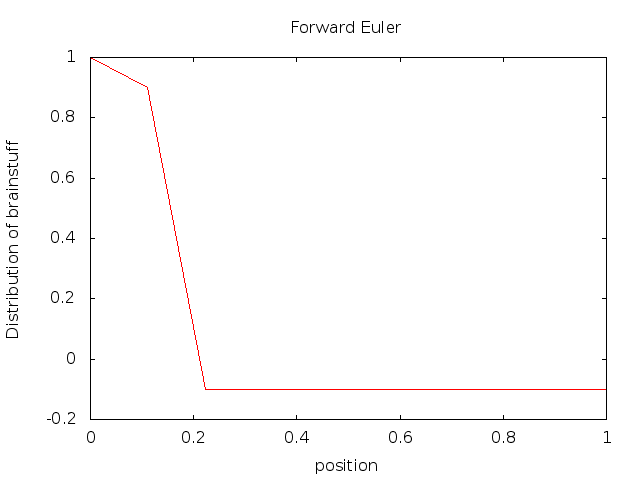
\includegraphics[width=0.5\textwidth]{Forwarddx101}
	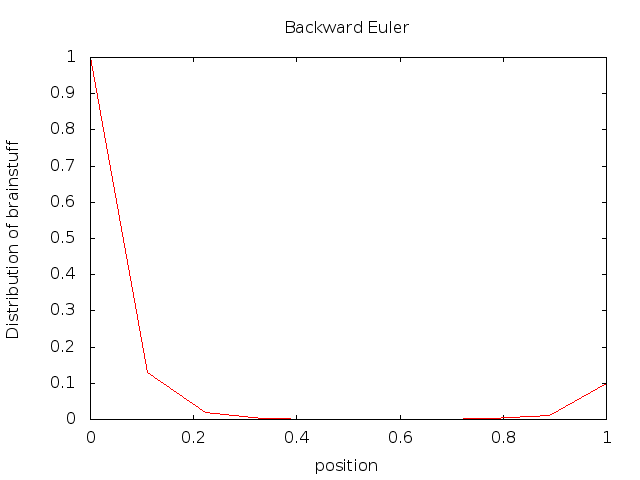
\includegraphics[width=0.5\textwidth]{Backwarddx101}
	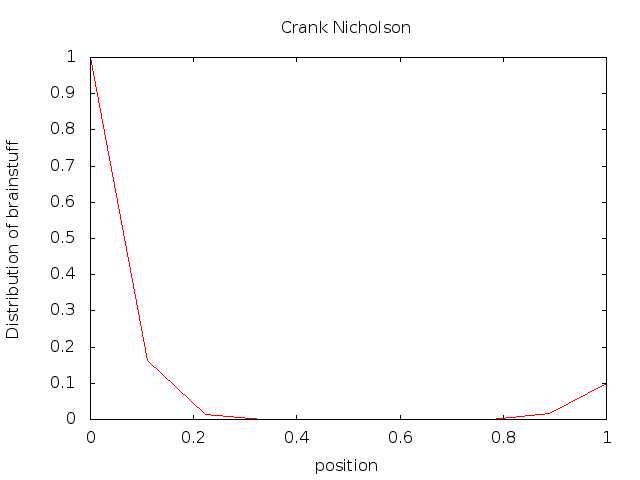
\includegraphics[width=0.5\textwidth]{Crankdx101}
	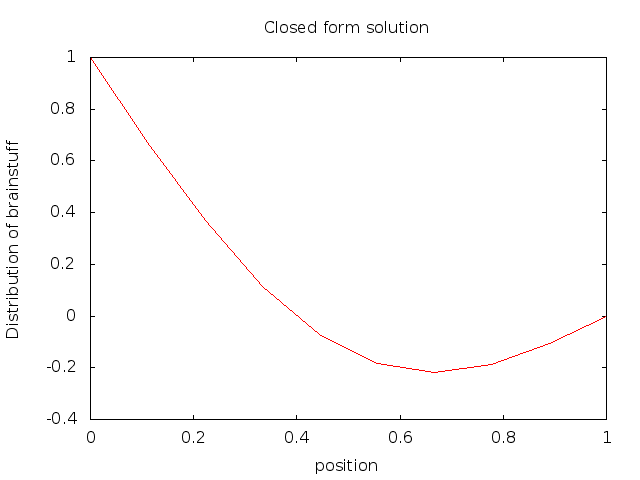
\includegraphics[width=0.5\textwidth]{Closedform1}
	\caption{The schemes and closed form solution after 1 time step for $\Delta x = 10$}
	\label{fig:01}
\end{figure}
\begin{figure}[hbtp]
	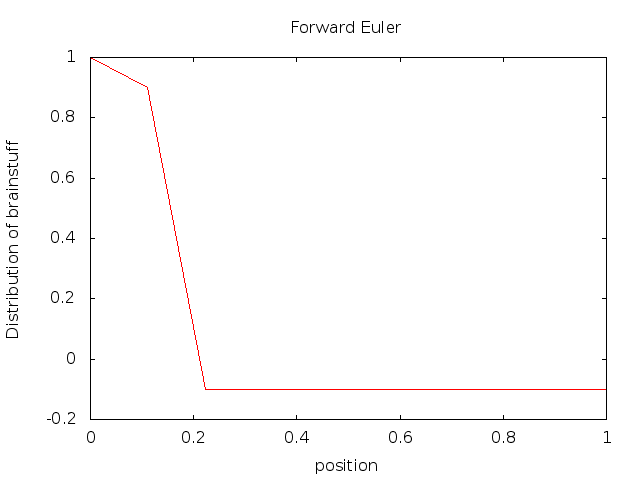
\includegraphics[width=0.5\textwidth]{Forwarddx10100}
	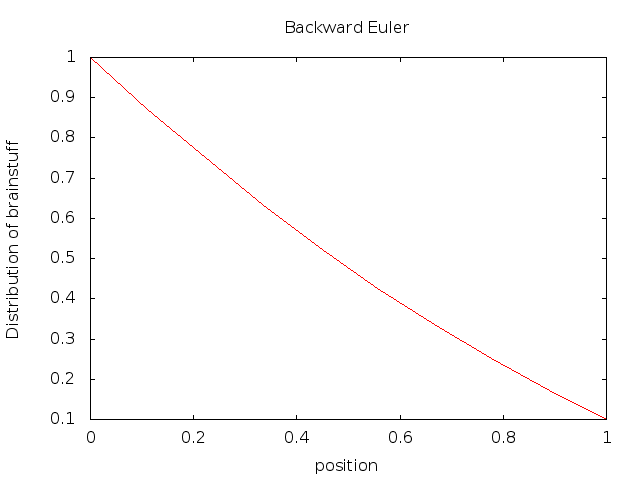
\includegraphics[width=0.5\textwidth]{Backwarddx10100}
	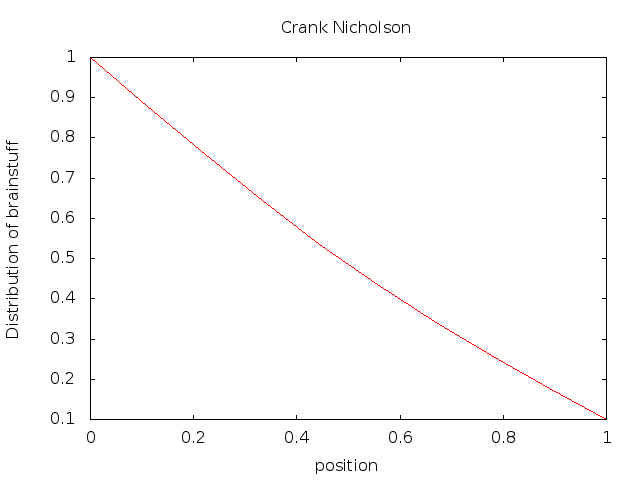
\includegraphics[width=0.5\textwidth]{Crankdx10100}
	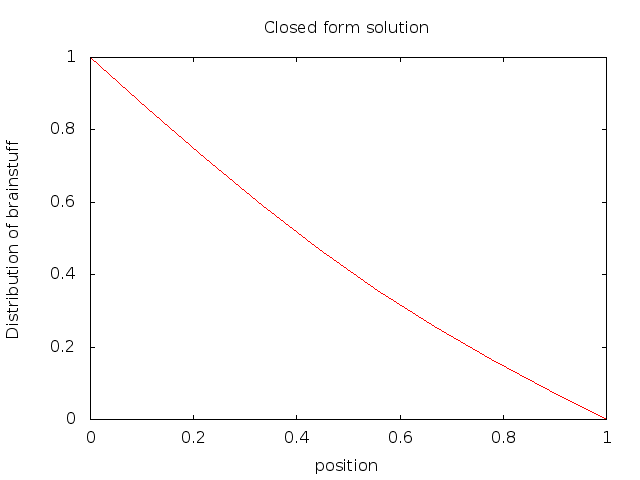
\includegraphics[width=0.5\textwidth]{Closedform10100}
	\caption{The schemes and closed form solution after 100 time step for $\Delta x = 10$}
	\label{fig:02}
\end{figure}
\begin{figure}[hbtp]
	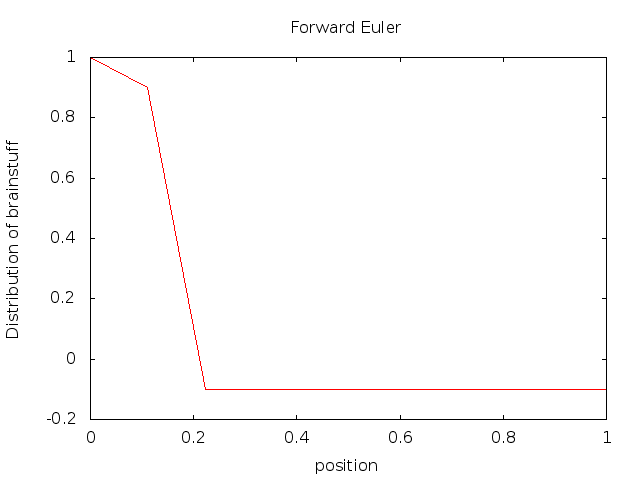
\includegraphics[width=0.5\textwidth]{Forwarddx101000}
	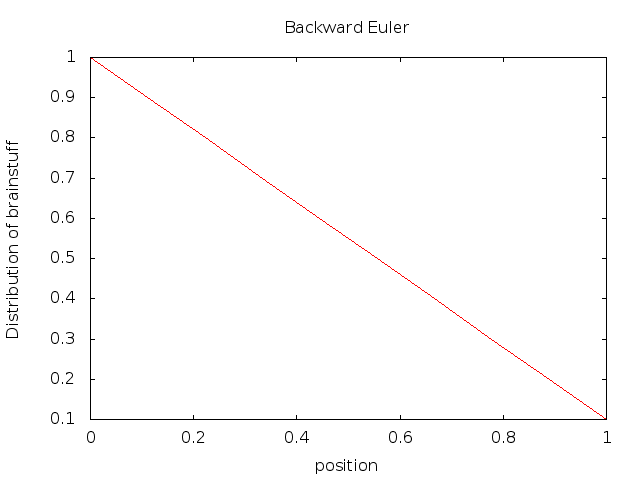
\includegraphics[width=0.5\textwidth]{Backwarddx101000}
	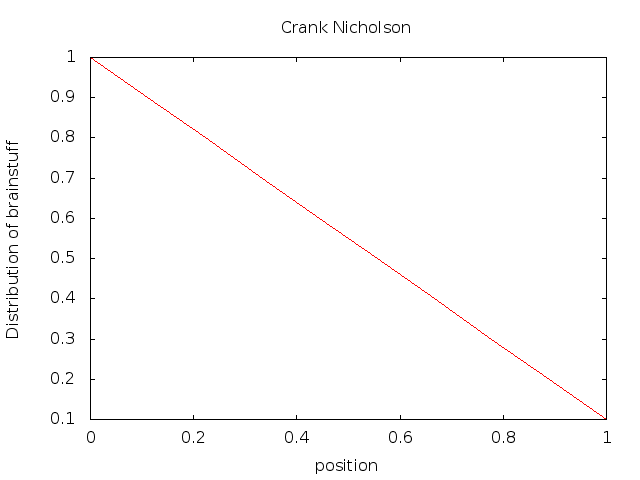
\includegraphics[width=0.5\textwidth]{Crankdx101000}
	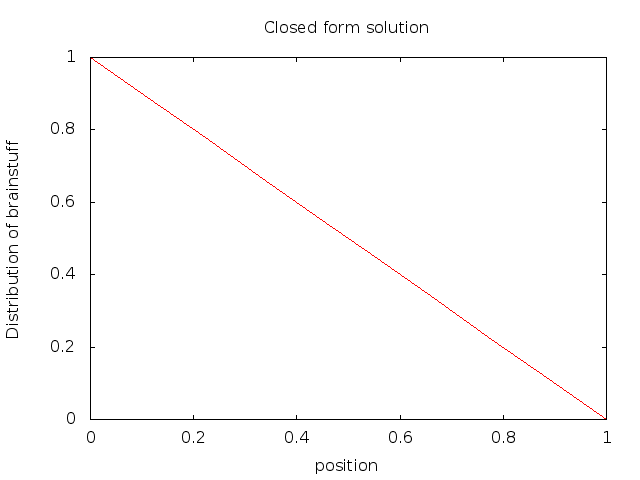
\includegraphics[width=0.5\textwidth]{Closedform101000}
	\caption{The schemes and closed form solution after 1000 time step for $\Delta x = 10$}
	\label{fig:03}
\end{figure}
\begin{figure}[hbtp]
	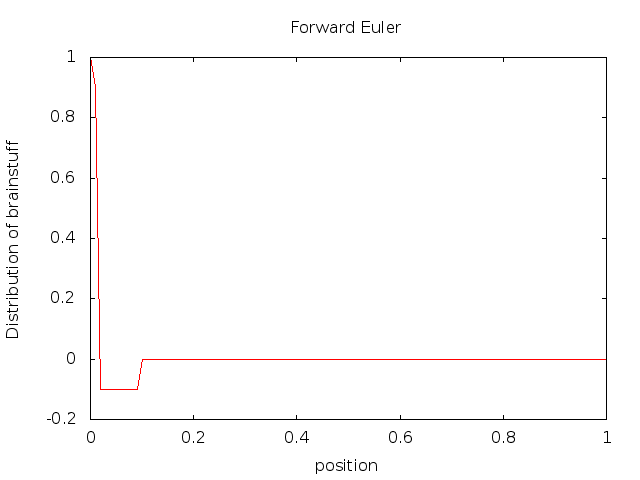
\includegraphics[width=0.5\textwidth]{Forwarddx1001}
	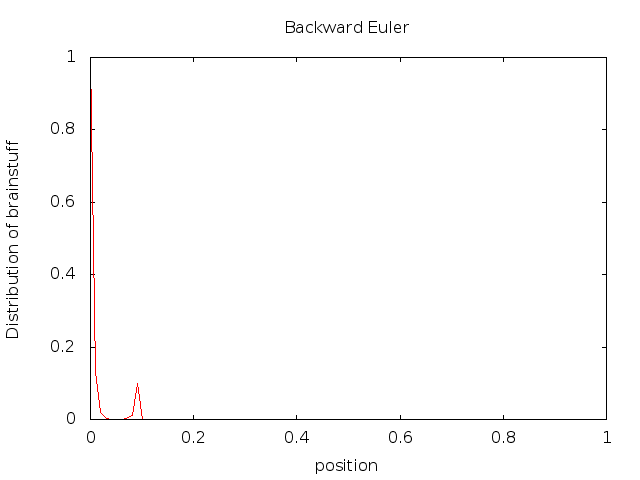
\includegraphics[width=0.5\textwidth]{Backwarddx1001}
	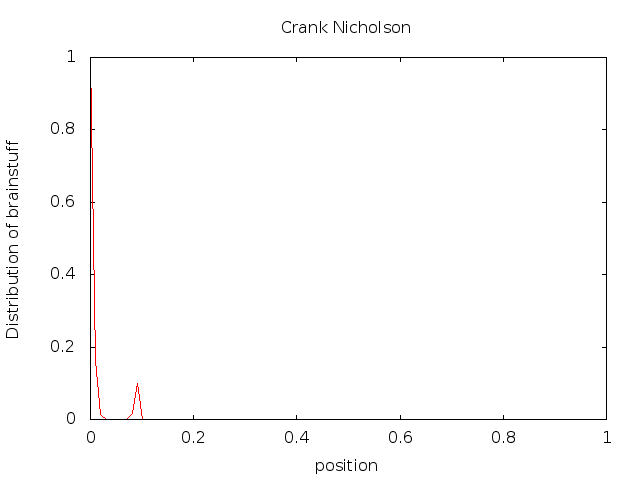
\includegraphics[width=0.5\textwidth]{Crankdx1001}
	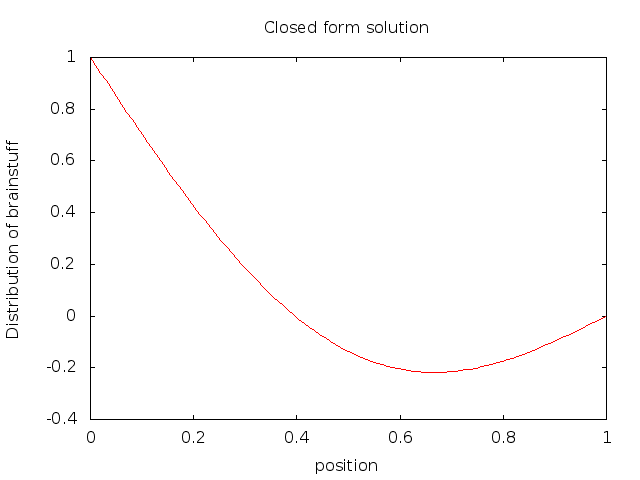
\includegraphics[width=0.5\textwidth]{Closedform1001}
	\caption{The schemes and closed form solution after 1 time step for $\Delta x = 100$}
	\label{fig:04}
\end{figure}
\begin{figure}[hbtp]
	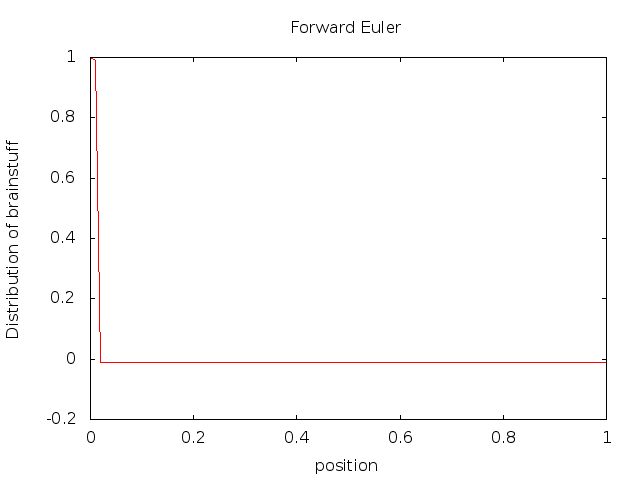
\includegraphics[width=0.5\textwidth]{Forwarddx100100}
	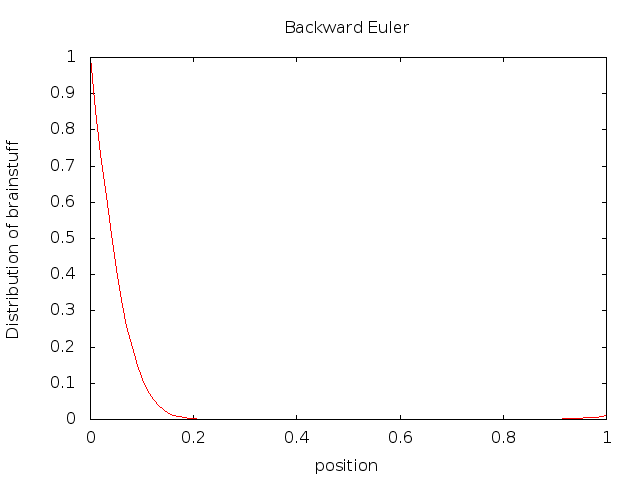
\includegraphics[width=0.5\textwidth]{Backwarddx100100}
	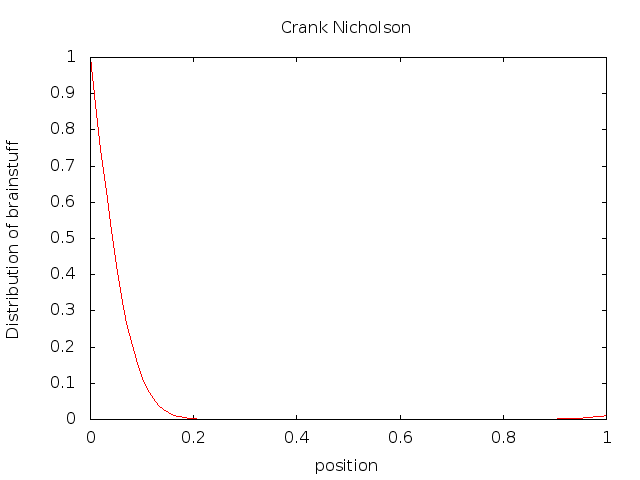
\includegraphics[width=0.5\textwidth]{Crankdx100100}
	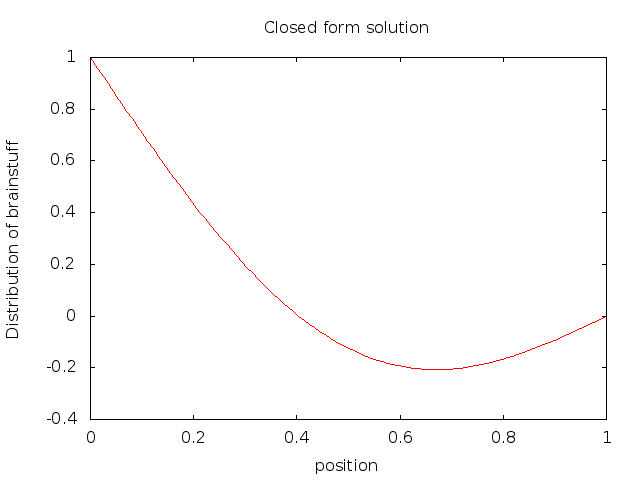
\includegraphics[width=0.5\textwidth]{Closedform100100}
	\caption{The schemes and closed form solution after 100 time step for $\Delta x = 100$}
	\label{fig:05}
\end{figure}
\end{document}








